\documentclass[../sparc.tex]{subfiles}
\graphicspath{{\subfix{../images/}}}
\begin{document}

%%%%%%%%%%%%%%%%%%%%%%%%%%%%%%%%%%%%%%%%%%%%%%%%%%%%%%%%%%%%%%%%%%%%%%%%%%%%%%%%
\section{Voltage}
\index{Electronics!Voltage}

Let's imagine that we have some vessel filled with water (see figure
\ref{fig:electronics-current-0}.)

\figureElectronicsVoltage{en}

The water in the vessel has some \emph{potential energy} that can be spent to
achieve some goal.  For example, if we make a hole in the bottom of the vessel
the water will be pouring down (as can be seen on
fig. \ref{fig:electronics-current-1}); if we put a waterwheel under the pouring
water we can use it as an engine for some mechanism.

\begin{figure}[ht]
  \centering
  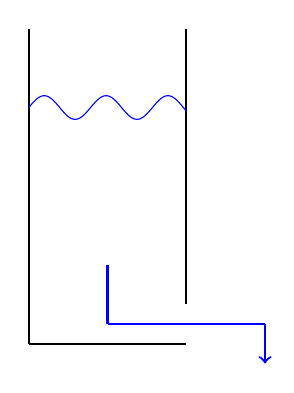
\begin{tikzpicture}[
      declare function={f1(\x) = 0.15 * sin(8.0 * deg(\x));
    }]

    \draw[thick] (0, 0) -- (0, 4);
    \draw[thick] (2, 0.5) -- (2, 4);
    \draw[thick] (0, 0) -- (2, 0);

    \draw[thick, color=blue] (1, 1) -- (1, 0.25);
    \draw[thick, color=blue] (1, 0.25) -- (3, 0.25);
    \draw[thick, color=blue, ->] (3, 0.25) -- (3, -0.25);

    \begin{scope}[yshift=3cm, color=blue]
      \draw (0, 0) plot[domain=0:2, variable=\x, samples=200, smooth] ({\x}, {f1(\x)});
    \end{scope}

  \end{tikzpicture}
  \caption{An example of a vessel with a hole in the bottom.}
  \label{fig:electronics-current-1}
\end{figure}

Drawing an analogy with the electricity we can say that our vessel has some
\emph{pressure} of water; in case of a charged electric battery we have some
``pressure'' of \emph{electrons}.  In case of the battery the energy is kept in
the form of \emph{chemical energy}.

The pressure of water is measured in \emph{Pascals} (Pa.)  The ``pressure'' of
electrons is measured in \emph{Volts} (V).

Thus we can draw our first conclusion: to make the electric current flow through
a circuit we have to have some current source that has some Voltage.

\end{document}
